\documentclass{beamer}
% \documentclass[handout,xcolor=pdftex,dvipsnames,table]{beamer}

\mode<presentation>
{
  \usetheme{Warsaw}
  \usecolortheme{whale}
  % or ...

  \setbeamercovered{transparent}
  % or whatever (possibly just delete it)
  \setbeamertemplate{navigation symbols}{}
}

\setbeamertemplate{itemize items}[ball]
\setbeamertemplate{itemize subitem}[triangle]
\setbeamertemplate{itemize subsubitem}[circle]
\setbeamercovered{transparent}

\usepackage{palatino} 
\usepackage{listings} % Gives syntax highlighting for python code. 
\usepackage{color} % Used for syntax highlighting. 
\usepackage{textcomp} % Used for syntax highlighting. 

% This gives syntax highlighting in the python environment 
\definecolor{gray}{gray}{0.5} 
\definecolor{key}{rgb}{0,0.5,0} 
\lstset{
language=python,
basicstyle=\ttfamily\tiny, 
otherkeywords={1, 2, 3, 4, 5, 6, 7, 8 ,9 , 0, -, =, +, [, ], (, ), \{, \}, :, *, !}, 
keywordstyle=\color{blue}, 
stringstyle=\color{red},
showstringspaces=false,
alsoletter={1234567890},
otherkeywords={\ , \}, \{},
keywordstyle=\color{blue},
emph={access,and,break,class,continue,def,del,elif ,else,%
except,exec,finally,for,from,global,if,import,in,is,%
lambda,not,or,pass,print,raise,return,try,while},
emphstyle=\color{black}\bfseries,
emph={[2]True, False, None, self},
emphstyle=[2]\color{green},
emph={[3]from, import, as},
emphstyle=[3]\color{blue},
upquote=true,
morecomment=[s]{"""}{"""},
commentstyle=\color{gray}\slshape,
emph={[4]1, 2, 3, 4, 5, 6, 7, 8, 9, 0},
emphstyle=[4]\color{blue},
literate=*{:}{{\textcolor{blue}:}}{1}%
{=}{{\textcolor{blue}=}}{1}%
{-}{{\textcolor{blue}-}}{1}%
{+}{{\textcolor{blue}+}}{1}%
{*}{{\textcolor{blue}*}}{1}%
{!}{{\textcolor{blue}!}}{1}%
{(}{{\textcolor{blue}(}}{1}%
{)}{{\textcolor{blue})}}{1}%
{[}{{\textcolor{blue}[}}{1}%
{]}{{\textcolor{blue}]}}{1}%
{<}{{\textcolor{blue}<}}{1}%
{>}{{\textcolor{blue}>}}{1},%
numbers=none,
}

\newcommand{\putat}[3]{\begin{picture}(0,0)(0,0)\put(#1,#2){#3}\end{picture}}

\title[]{Python Workshop\\
Numpy Arrays}

\author[Langevin] % (optional, use only with lots of authors)
{C.D.~Langevin}
\institute[USGS] % (optional, but mostly needed)
{
  U.S. Geological Survey\\
  Reston, Virginia, USA
  }

\titlegraphic{
\includegraphics[scale=0.5]{figures/c_USGSid1.pdf}}

\date[UQ12] % (optional, should be abbreviation of conference name)
{USGS National Groundwater Workshop, August 2012}

\subject{Python}


\begin{document}

\begin{frame}
  \titlepage
\end{frame}

%put this pdf image on all following slides
\logo{\vspace{-0.3cm} 
\includegraphics[width=1.5cm]{figures/c_USGSid1.pdf}\hspace*{11.10cm}}  

\begin{frame}{Outline}
\tableofcontents
\end{frame}

\section{Numpy Arrays}
\begin{frame}[fragile]
\frametitle{What is Numpy}
\begin{itemize}
  \item Numpy is the main package for scientific computing using Python
  \item Provides an array object of type ndarray
  \item Many functions and methods available for fast array operations
\end{itemize}
\end{frame}

\begin{frame}[fragile]
\frametitle{Numpy Version}
\begin{itemize}
  \item Numpy can be obtained at \url{http://docs.scipy.org/doc/}
  \item Current version is 1.6.
  \item To determine the installed version
\end{itemize}
  \begin{lstlisting}
In [10]: import numpy

In [11]: print numpy.__version__
1.6.1
  \end{lstlisting}
\end{frame}


\begin{frame}[fragile]
\frametitle{Data Types (dtype)}
\begin{table}
\tiny
\begin{tabular}{l l}
  bool        & Boolean (True or False) stored as a byte                                         \\
  int         & Platform integer (normally either int32 or int64)                                \\
  int8        & Byte (-128 to 127)                                                               \\
  int16       & Integer (-32768 to 32767)                                                        \\
  int32       & Integer (-2147483648 to 2147483647)                                              \\
  int64       & Integer (9223372036854775808 to 9223372036854775807)                             \\
  uint8       & Unsigned integer (0 to 255)                                                      \\
  uint16      & Unsigned integer (0 to 65535)                                                    \\
  uint32      & Unsigned integer (0 to 4294967295)                                               \\
  uint64      & Unsigned integer (0 to 18446744073709551615)                                     \\
  float       & Shorthand for float64.                                                           \\
  float16     & Half precision float: sign bit, 5 bits exponent, 10 bits mantissa                \\
  float32     & Single precision float: sign bit, 8 bits exponent, 23 bits mantissa              \\
  float64     & Double precision float: sign bit, 11 bits exponent, 52 bits mantissa             \\
  complex     & Shorthand for complex128.                                                        \\
  complex64   & Complex number, represented by two 32-bit floats (real and imaginary components) \\
  complex128  & Complex number, represented by two 64-bit floats (real and imaginary components) \\ 
\end{tabular}
\end{table}
\url{http://docs.scipy.org/doc/numpy-1.6.0/user/basics.types.html}
\end{frame}

\begin{frame}[fragile]
\frametitle{Creating an Array}
\begin{itemize}
  \item{Using the built-in array function}
  \begin{lstlisting}
In [18]: import numpy

In [19]: a1d = numpy.array([0, 1, 2, 3, 4])

In [20]: a1d
Out[20]: array([0, 1, 2, 3, 4])

In [21]: a2d = numpy.array([ [1, 1, 1, 1], [2, 2, 2, 2] ])

In [22]: a2d
Out[22]:
array([[1, 1, 1, 1],
       [2, 2, 2, 2]])
  \end{lstlisting}
  \item Using the arange built-in function
  \begin{lstlisting}
In [25]: a = numpy.arange(10)

In [26]: a
Out[26]: array([0, 1, 2, 3, 4, 5, 6, 7, 8, 9])

In [27]: a = numpy.arange(0, 100, 10)

In [28]: a
Out[28]: array([ 0, 10, 20, 30, 40, 50, 60, 70, 80, 90])
  \end{lstlisting}
\end{itemize}
\end{frame}

\begin{frame}[fragile]
\frametitle{Creating an Array}
\begin{itemize}
  \item{Using the built-in linspace function}
  \begin{lstlisting}
In [29]: a = numpy.linspace(0, 1, 7)

In [30]: a
Out[30]:
array([ 0.        ,  0.16666667,  0.33333333,  0.5       ,  0.66666667,
        0.83333333,  1.        ])
  \end{lstlisting}

  \item{Creating a new array from an existing array using a numpy function}
  \begin{lstlisting}
In [16]: import numpy

In [17]: x = numpy.linspace(0, 2 * numpy.pi, 20)

In [18]: y = numpy.sin(x)

In [19]: plot(x, y)
Out[19]: [<matplotlib.lines.Line2D object at 0x04A7B8B0>]

In [20]: show()
  \end{lstlisting}

\end{itemize}
\end{frame}

\begin{frame}[fragile]
\frametitle{Loading an Array from a File}
  \centering
    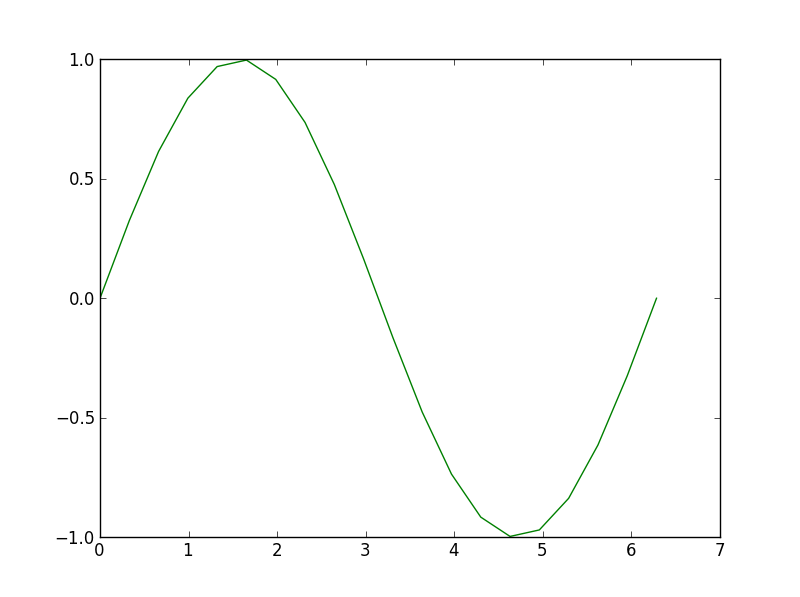
\includegraphics[width=1.\textwidth]{figures/sinx.png} 
\end{frame}

\begin{frame}[fragile]
\frametitle{Loading an Array from a File}
\begin{itemize}
\item{If we have the following table stored in an ascii text file}
\begin{tabular}{l l l l}
  1 & 3 & 6 & 9 \\
  12 & 15 & 18 & 21 \\
  23 & 26 & 29 & 31 \\
  77 & 78 & 79 & 2 \\
\end{tabular}
\item{The table can be loaded into a numpy array using the numpy loadtxt function}
\begin{lstlisting}
In [28]: a = numpy.loadtxt('data\\4by4array.txt')

In [29]: a
Out[29]:
array([[  1.,   3.,   6.,   9.],
       [ 12.,  15.,  18.,  21.],
       [ 23.,  26.,  29.,  31.],
       [ 77.,  78.,  79.,   2.]])
\end{lstlisting}
\end{itemize}
\end{frame}

\begin{frame}{Theis Example}
  \small{\texttt{theis.py}}
  \begin{figure}[ht]
  \centering
        \lstset{numbers=left}
        \lstinputlisting[language=python, firstnumber=1]{python/theis.py}
   \end{figure}
   \putat{200}{20}{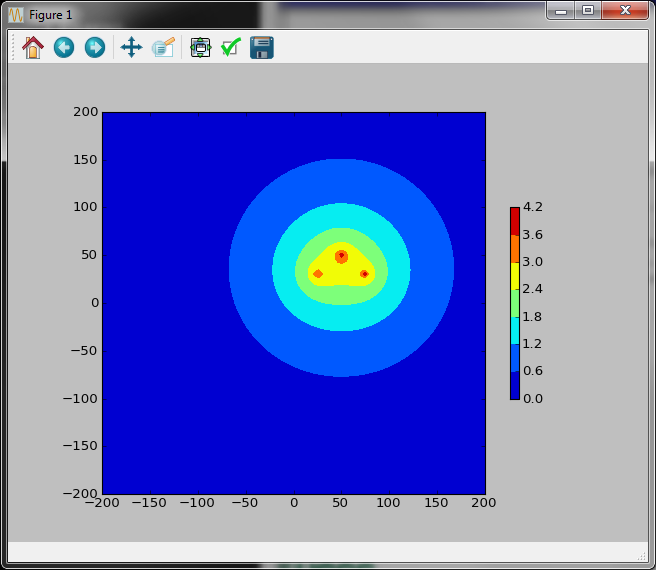
\includegraphics[width=4.5cm]{figures/theis.png} }
\end{frame}

\begin{frame}[fragile]
\frametitle{Indexing, Slicing, and Iterating}
\end{frame}

\begin{frame}[fragile]
\frametitle{Shape Manipulation}
\end{frame}

\end{document}